\documentclass[10pt,twocolumn,letterpaper]{article}

\usepackage{cvpr}
\usepackage{times}
\usepackage{epsfig}
\usepackage{graphicx}
\usepackage{amsmath}
\usepackage{amssymb}
\usepackage{booktabs}
\usepackage{microtype}
% From https://ctan.org/pkg/matlab-prettifier
\usepackage[numbered,framed]{matlab-prettifier}
\usepackage{pythonhighlight}

\frenchspacing

% Include other packages here, before hyperref.

% If you comment hyperref and then uncomment it, you should delete
% egpaper.aux before re-running latex.  (Or just hit 'q' on the first latex
% run, let it finish, and you should be clear).
\usepackage[pagebackref=true,breaklinks=true,letterpaper=true,colorlinks,bookmarks=false]{hyperref}

\cvprfinalcopy % *** Uncomment this line for the final submission

\def\cvprPaperID{****} % *** Enter the CVPR Paper ID here
\def\httilde{\mbox{\tt\raisebox{-.5ex}{\symbol{126}}}}

% Pages are numbered in submission mode, and unnumbered in camera-ready
\ifcvprfinal\pagestyle{empty}\fi
\begin{document}

%%%%%%%%% TITLE
\title{CSCI 1430 Final Project Report:\\Immersive Panorama Stitching and Visualizing}

\author{\emph{SHAKSHUKA}: Marina Triebenbacher, Zachary Mothner, William Buerger, Rachel Yan.\\
Brown University\\
9 May 2020
}

\maketitle
%\thispagestyle{empty}

%%%%%%%%% BODY TEXT
\section{Introduction}

Drawing inspiration from Google Arts and Culture, as well as the inordinate amount of time we now spend in our rooms, our group aimed to build a panoramic viewing experience of our rooms in quarantine.

In order to build a 360 degree panorama, we first projected images taken with a calibrated camera onto cylindrical coordinates, then stitched them together to create the panorama. We then used \textbf{some} blending to smooth the seams of the image. Finally, we built a flexible panorama viewer that provides an interactive virtual view of the 360 degree panorama.

\section{Related Work}

We leaned on many helpful resources to achieve our final results. This Learn OpenCV~\cite{sadekar20} article was integral in helping us calibrate our cameras. We thank Yun Miao~\cite{miao12} for his extremely insightful final project report for Brown's Computational Photography course, which led us to Professor Dyer's slides on inverse cylindrical projection equations~\cite{dyer}. This Applet~\cite{dektar12} showed many useful visualization of both cylindrical panoramas and planar reprojections, and we only dream to have achieved a product as cool as this one. Finally, a myriad of Powerpoint slides by professors around the country helped round out our research, such as this one~\cite{kari10} from Stanford Graphics, which outlined 360 panoramas, and this one~\cite{seitz} from Columbia, which detailed the homography matrix for a shift translation.

\section{Method}

We began by attempting to stitch together planar images with traditional methods: using SIFT as the feature extractor, a KNN feature matcher, and RANSAC to estimate the homography matrix. Then, we used OpenCV's warpPerspective() to apply a perspective transformation to one of the images, successfully stitching them together. While this method initially seemed promising, we quickly realized that it was not possible to achieve a 360 degree panorama using planar images and perspective reprojection.

Our next step was to build a cylindrical panorama: project each image onto a cylinder, then reproject a portion of the cylinder onto a 'display screen' in our visualizer.\\\\
\textbf{Step 1: Camera Calibration}

Because knowing the focal length of our camera is necessary to compute the cylindrical projection, we used this OpenCV Camera Calibration tutorial~\cite{sadekar20} as well as a 7x9 checkerboard to calibrate an iPhone camera.

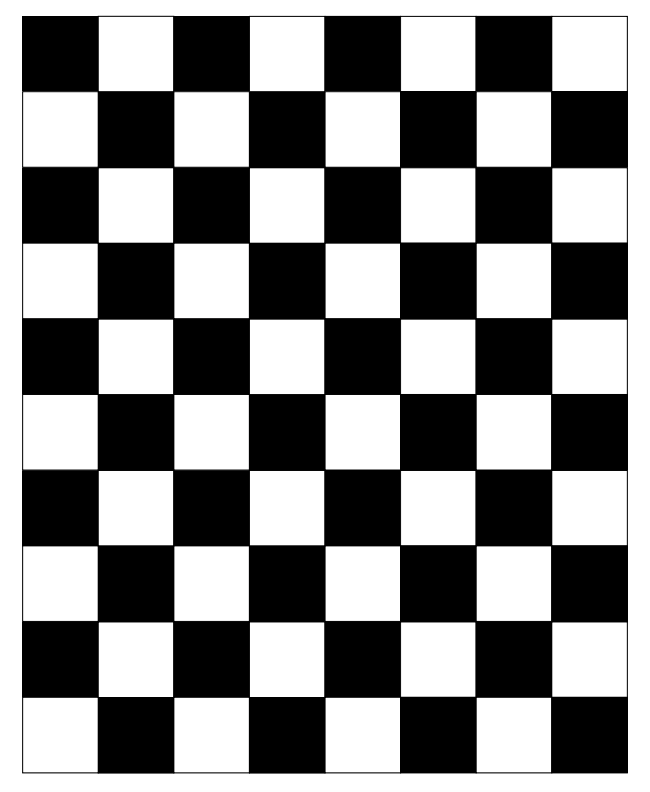
\includegraphics[width=4cm]{checkerboard.png}

First we define real world coordinates by photographing this checkerboard with known dimensions at different orientations. Because all corner points of the checkerboard lie on a plane and are equally spaced apart, we can use the known 3D world coordinates of the checkerboard to locate the 2D pixel locations in the images. Passing these two sets of coordinates into openCV's calibrateCamera() results in the intrinsic matrix of our calibrated camera.\\\\
\textbf{Step 2: Projecting to Cylindrical Coordinates}

We used this slide deck from UWisc Professor Charles Dyer~\cite{dyer} to calculate inverse cylindrical projections for the images. The following equations were used to calculate the cylindrical coordinates from the planar coordinates:
\begin{align}
\theta &= (x_{cyl} - x_c)/f\\
h &= (y_{cyl} - y_c)/f\\
\hat{x} &= sin\theta \\
\hat{y} &= h \\
\hat{z} &= cos\theta \\
x &= f\hat{x}/\hat{z} + x_c \\
y &= f\hat{y}/\hat{z} + y_c
\label{eq:cylindrical}
\end{align}
where $\hat{x}, \hat{y}, \hat{z}$ are the cylindrical coordinates and $x, y$ are the planar reprojections. This code snippet demonstrates the calculations for a single pixel:
\begin{python}
theta = (x_cyl - x_c) / f
h = (y_cyl - y_c) / f
X = np.array([math.sin(theta), h, 
    math.cos(theta)])

# Calculates the warped X pixel location
x_im = (f * (X[0]/X[2])) + x_c
if x_im < 0 or x_im >= width:
    continue
    
# Calculates the warped y pixel location
y_im = (f * (X[1]/X[2])) + y_c
if y_im < 0 or y_im >= height:
    continue
    
# If both pixel values are in bounds, 
# store it in the cylindrical location
cyl[int(y_cyl),int(x_cyl)] 
    = img[int(y_im),int(x_im)]
\end{python}

\bigskip
\noindent\textbf{Step 3: Stitching the Cylindrical Images}\\

First, we use SIFT to find and return all of the features in the images, OpenCV's Brute Force matcher to find the best feature matches, and RANSAC to generate the homography matrix based on the feature matches.

For cylindrical projections, the only 2D geometric translation we have to take into account is a translation. From this presentation by Professor Peter K. Allen~\cite{seitz}, we found that the homography matrix is 
\[
  \left[ {\begin{array}{ccc}
   1 & 0 & t_x\\
   0 & 1 & t_y\\
   0 & 0 & 1
  \end{array} } \right],
\]
where $t_x$ represents horizontal translation and $t_y$ represents vertical translation. Therefore, given the homography matrix, we can obtain the horizontal and translational shift of the images and stitch together accordingly. The following code shows stitching of two images given the images and shift:\\\\
\begin{python}
def stitch(img1, img2, shift):
    shift[0] = int(shift[0])
    shift[1] = int(shift[1])
    # Pads the left image to account for 
    vertical shift
    padding = [ (int(shift[0]), 0) 
        if shift[0] > 0 
        else (0, int(-shift[0])),
        (0,0),(0,0)]
    shifted_img1 = np.lib.pad(img1, padding, 
        'constant', constant_values=0)
    # Gets the horizontal and verticle shift 
    to splice the first image
    horiz = int(shifted_img1.shape[1]) - 
        int(abs(shift[1]))
    vert = int(abs(shift[0]))
    shifted_img1 = shifted_img1[vert:, :horiz]
    # Concatenates the splices left image 
    to the right image
    stitched = np.concatenate(
        (shifted_img1, img2), axis=1)
    return stitched
\end{python}

\bigskip
\noindent\textbf{Step 4: Creating the Panorama Visualizer}

We built the 360 panorama visualizer using the Python libraries PIL, for image processing, and TKinter, for graphical displays. The visualizer takes any type of image, automatically adjusts the window size for an appropriate display, and uses user input from the four arrow keys to pan around the image.

In addition to basic four-directional movement, it was important to us to have the ability to wrap around our 360 panoramas continuously, providing an immersive experience, as if someone is turning in a constant circle around the space. The visualizer tracks the horizontal and vertical shifts around the image and whenever the visualizer is initialized with wrapping set to True, it automatically wraps along where the edges of the image would be. To the user, there is no evidence of any edges, appearing like a continuous image (relying on a well-made panorama).

\section{Results}

Our initial result of stitching together planar images was relatively successful (Figure \ref{fig:result1}) but the strategy could not be extended to 360 degree panoramas.

\begin{figure}[h]
    \centering
    % \includegraphics[width=\linewidth]{bed-result.jpeg}
    \caption{Planar Stitching Result.}
    \label{fig:result1}
\end{figure}

Once we had a calibrated camera, we were able to take a series of images with $>25\%$ overlap using a tripod and convert each one to cylindrical coordinates. Figure \ref{fig:result2} shows an example planar image with its cylindrical counterpart.\\

\pagebreak

\begin{figure}[h]
    \centering
    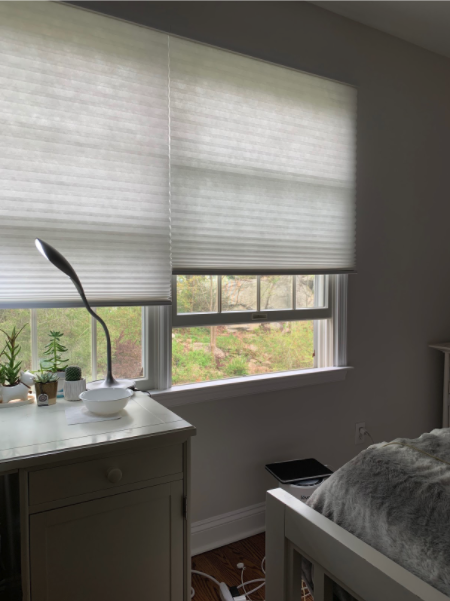
\includegraphics[width=0.5\linewidth]{noncylindrical.png}
    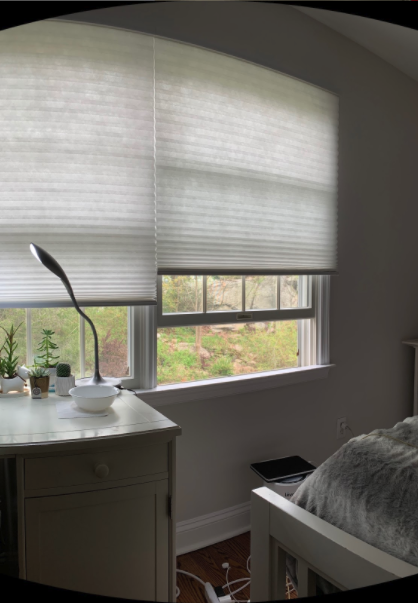
\includegraphics[width=0.465\linewidth]{cylindrical.png}
    \caption{\emph{Left:} Original Image. \emph{Right:} Warped Image reprojected from cylindrical coordinates.}
    \label{fig:result2}
\end{figure}

Finally, using the techniques we learned in class (SIFT, matching, RANSAC), we achieved a 360 degree panorama image. Figure \ref{fig:result3} displays this result.
\begin{figure}[h]
\centering
 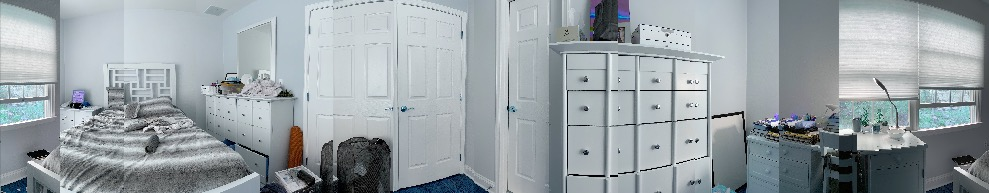
\includegraphics[width=\linewidth]{pano5.jpg}
\caption{Stitched 360 degree panorama. }
\label{fig:result3}
\end{figure}

%-------------------------------------------------------------------------
\subsection{Discussion}

While our method was roundabout, we believe we ended up taking the right approach in constructing a 360 degree panorama. Our stitched result could be greatly improved with seam removing and image blending, which we toyed around with but couldn't quite get to work. The graph cut algorithm, as well, could be used to remove seams. In terms of the visualizer, we could've introduced smoother panning and zooming capabilities to enhance the immersive feeling. Given our limited time, resources, and computer vision knowledge, however, we are generally satisfied with our results.

%------------------------------------------------------------------------
\section{Conclusion}

As the weeks of isolation wore on, our project, meant initially as a reflection of our time at home, ironically became a means of connecting us together. We are so used to navigating the dialectical relationship between solitude and socialization, that it is jarring to suddenly be in one state all the time. Our lives, which were completely in sync, have been abruptly torn apart. It's impossible to generalize what this experience is like for anyone else — we know all four of us are extraordinarily privileged compared to the rest of the country, yet even we are experiencing quarantine differently. This project symbolizes multiple conflicting feelings: it's about choosing to root ourselves in the nature of the place we're in, even if we're here by necessity; it's an invitation for others to take a little part in our quarantine experience; and the reality of the project in and of itself was a source of connection and socialization.

{\small
\bibliographystyle{plain}
\bibliography{bibliography}
}

\section*{Appendix}

\subsection*{Team contributions}
\begin{description}
\item[Marina] Definitely took the lead on this project and completed the bulk of the research and code on cylindrical warping and stitching (the pictures are of her bedroom!)

\item[Zach] Worked on planar stitching and cropping in the early stages of the project, contributed to the presentation, and worked on blending.

\item [Will] Wrote the entire panorama visualizer as well as many of the weekly progress reports. Spoke for our team in the presentation. 

\item [Rachel] Worked initially on planar feature matching and stitching. Did some research on inverse cylindrical coordinates, and wrote the writeup.
\end{description}

\end{document}